\section{Algebra}
\label{sec:algebra}

In this section we describe the operators of \tg algebra.  The algebra
is compositional --- all operators take a \tg or a pair of \tgs as
input, and produce a valid \tg as output.

\subsection{Preliminaries}
\label{sec:algebra:prelim}

B\"ohlen et al.~\cite{DBLP:conf/vldb/BohlenSS96} show that temporal
selection, Cartesian product and difference all produce a coalesced
relation as output if the input was coalesced.  They also show that
temporal union and temporal projection can give rise to an uncoalesced
output even if the inputs were coalesced.  Intuitively, this is
because union and projection can give rise to duplicates in
traditional relational algebra, and lack of coalescing is the temporal
analogy to a duplicate.

These observations also hold in our scenario at the level of
individual relations, each containing representative graphs, vertices,
edges, or vertex/edge attributes.

Our algebra operates on \tgs, and so, in addition to keeping the data
structure (and its constituent parts) coalesced, we must ensure that
the result is a valid \tg.\eat{ This objective informed our design of
  the algebra, e.g., we did not include some flavors of temporal
  aggregation because the result would be invalid.  Further, this
  objective informs the rewriting of applicable operations over the
  \ve representation.}  Importantly, when manipulating the \ve
representation, we do not require that each intermediate state of the
data structure correspond to a valid \tg, but rather that the final
result, which is usually derived after several steps, be valid.  To
have a useful algebra, we do not reject a change that would lead to a
violation in referential integrity.  Instead, we compute a consistent
result by removing the tuples that violate referential integrity.

Our algebra is based on the principle of snapshot
reducibility~\cite{DBLP:reference/db/Bohlen092}.  This principle
states that an operation should yield the same result when applied to
the temporal representation as it would if it were applied separately
to every snapshot state of the temporal representation.

Consider a unary operation \opp and suppose that it is being evaluated
over the \ve representation \opp(\tve).  Algorithm~\ref{alg:op}
outlines the steps in the evaluation, overloading \opp as appropriate
when applying the operation to constituent parts of \tve.  Some of the
steps in Algorithm~\ref{alg:op} may be unnecessary because of the
properties of the particular operation, as we will see in the
remainder of this section.  Furthermore, some of the operations may
produce correct results (up to coalescing) {\em even when computing
  over uncoalesced inputs}.  This was discussed in the context of
temporal relational algebra in~\cite{DBLP:conf/vldb/BohlenSS96}, and
rules were proposed to eliminate superfluous coalescing. We will
revisit this point in the context of \tg algebra when discussing lazy
evaluation in Section~\ref{sec:sys:coal}.

\begin{algorithm}[h!]
\caption{Evaluation of a unary operation \opp on \tve}
\begin{algorithmic}[1]
\REQUIRE \tg $\tve (\tv; \te; \tav; \tae)$, operation \insql{op}.\\
\STATE  $\tv' = \cl (\opp(\tv))$\\
\STATE  $\te' = \cl (\opp(\te))$\\
\STATE  $\tav' = \cl (\opp(\tav))$\\
\STATE  $\tae' = \cl (\opp(\tae))$\\
\STATE  enforce foreign keys on $\te'$ w.r.t. $\tv'$\\
\STATE  enforce foreign keys on $\tav'$ w.r.t. $\tv'$\\
\STATE  enforce foreign keys on $\tae'$ w.r.t. $\te'$\\
\RETURN new $\tve (\tv';\te';\tav';\tae')$\\
\end{algorithmic}
\label{alg:op}
\end{algorithm}

\subsection{Slice}
\label{sec:algebra:slice}

The unary {\em slice} operator, denoted $\tau_c (T)$, where $c$ is a
time period, cuts a temporal slice from $T$.  The resulting \tg will
contain representative graphs whose period $p$ has a non-empty
intersection with $c$ (i.e., $p$ is either contained within $c$ or
overlaps with it, see Section~\ref{sec:model:prelim}).  If $p.start <
c.start$ or $p.end > c.end$ for some tuple $(g, p)$, then $p$ is
trimmed to be within the boundaries of $c$: $\tau_c (\trg) = \{ (g, p
\cap c)~~|~~(g, p) \in \trg \wedge (\pred{c}{overlaps}{p} \vee
\pred{c}{contains}{p})\}$.

To evaluate $\tau_c (\tve)$, we apply $\tau_c$ to each of the four
constituent relations of \tve.  For example: 
$\tau_c (\tv) = \{ (v, p
\cap c)~~|~~(v, p) \in \tv \wedge (\pred{c}{overlaps}{p} \vee \pred{c}{contains}{p}) \}$, 
and analogously for each \te, \tav and \tae.

\eat{ 
In SQL, slice can be expressed as follows for $V$ (similarly for other
relations):}

\eat{\begin{small}
\begin{verbatim}
SELECT vid, a1, ..., an, greatest(estart, DATE ':date1'), 
       least(eend, DATE ':date2')
FROM V
WHERE eperiod OVERLAPS PERIOD (DATE ':date1', DATE ':date2')
\end{verbatim}
\end{small}}

{\bf Slice does not uncoalesce.} Whether evaluated over \trg or \tve,
slice is guaranteed to return a coalesced relation when evaluated over
a coalesced input.  This is because, for any relation \insql{R}, there
will be at most one tuple from \insql{R} in the result of $\tau_c (R)$,
with a validity period that is either the same as it was in \insql{R},
or further restricted (trimmed).  Therefore, there is no need to
coalesce \trg after slice, or on lines 1-4 of Algorithm~\ref{alg:op}
when operating over \tve.

{\bf Slice does not require FK enforcement for \tve.}  To see why,
consider an edge $\te(v_1, v_2, p)$ and one of the corresponding
vertices $\tv(v_1, p_1)$, such that $\pred{p_1}{contains}{p}$ (per
Definition~\ref{def:tg} condition~\ref{def:tg:c1}).  Suppose now that
slice was applied to \tv and to \te with condition $c$.  Is it
possible that edge $(v_1, v_2, p \cap c)$ is in the result of $\tau_c
(\te)$ (i.e., $p \cap c \neq \emptyset$), while vertex $\tv(v_1, p_1 \cap
c)$ is not in the result of $\tau_c (\tv)$ (i.e., $p_1 \cap c =
\emptyset$)?  Clearly, the answer is no, since
$\pred{p_1}{contains}{p}$, and so it must be the case that
$\pred{p_1}{contains}{(p \cap c)}$.  A similar argument justifies that
FK enforcement is not needed for $\tau_c(\tav)$ (w.r.t. $\tau_c (\tv)$) and
for $\tau_c(\tae)$ (w.r.t. $\tau_c (\te)$).

\subsection{Temporal subgraph matching}
\label{sec:algebra:subgraph}

Temporal subgraph matching is defined analogously to subgraph matching
in non-temporal graphs: it applies a subgraph function $f$ to every
representative graph of the input.  To ensure that a valid \tg is
computed as a result of this operation, we restrict our attention to
functions that compute a single subgraph of a given representative
graph as a result: $\sigma_f (\trg) = \{ (g', p)~~|~~(g, p) \in \trg
\wedge g' = f(g) \wedge$\\$V_{g'} \subseteq V_{g} \wedge E_{g'}
\subseteq E_{g} \}$.

\eat{For example, $f$ may select a subset of the vertices or edges of
  $g$ based on some condition that can be computed locally at a vertex
  or edge, or by a path / reachability expression.  In this paper we
  restrict our attention to conjunctive queries.}  Even more
specifically, we focus on functions that can be expressed as a pair of
{\em conjunctive queries} $\sigma_{C_V,C_E} (\trg)$, where $C_V$
specifies {\em non-temporal predicates} over the vertices of $g$, and
$C_E$ --- over the edges of $g$. (Computing arbitrary subgraphs of an
evolving graph is beyond the scope of this paper, and we defer this to
future work.)

Like other unary operators, $\sigma_{C_V, C_E} (\tve)$ follows the
outline of Algorithm~\ref{alg:op}.  Importantly, since $C_V$ and $C_E$
may involve predicates over the attributes, we compute the join of the
vertex (resp. edge) relation with the corresponding attribute relation
to evaluate the query, and push selections as appropriate.  Line 1 of
Algorithm~\ref{alg:op} becomes: $\tv' = \pi_{v,p} (\sigma_{C_{V1}} (V)
\bowtie \sigma_{C_{V2}} (\tav))$.  Similarly, we compute $\te' =
\pi_{v_1,v_2,p} (\sigma_{C_{E1}} (E) \bowtie \sigma_{C_{E2}} (\tae))$
(line 2), $\tav' = \sigma_{C_{V2}} (\tav)$ (line 3) and $\tae' =
\sigma_{C_{V2}} (\tae)$ (line 4).

{\bf Subgraph does not uncoalesce \tve.}  Consider again the
computation of $\tv'$ described above, with a query that involves
projection, selection and join over temporal SQL relations $\tv$ and
\tav.  While selection and join cannot produce an uncoalesced output
if the input is coalesced, projection may produce an uncoalesced
output relation~\cite{DBLP:conf/vldb/BohlenSS96}.  Interestingly,
projection does not result in an uncoalesced output in this case. To
see why, suppose that $C_V$ is trivial, i.e., that $\sigma_{C_{V1}}
(\tv) = \tv$ and $\sigma_{Q_{C2}} (\tav) = \tav$. Then $\tv' =
\pi_{v,p} (\tv \bowtie \tav)$, and since $\tv \bowtie \tav$ is a
primary key-foreign key join, then $\tv' = \tv$.  If $C_V$ is
non-trivial, i.e., $\sigma_{Q_{C1}} (\tv) \subset \tv$ or
$\sigma_{C_{V2}} (\tav) \subset \tav$, then it will be the case that
$V' \subset V$.  In both cases, if $\tv$ is coalesced then so is
$\tv'$.  A similar argument applies to the edges relation $\te'$.
Finally, since $\tav'$ and $\tae'$ are computed from coalesced input
relations using only selection, they are guaranteed to be coalesced.
Thus, it is not necessary to coalesce on lines 1-4 of
Algorithm~\ref{alg:op}.

{\bf Subgraph does require FK enforcement for \tve.}  Perhaps the most
natural temporal subgraph query is one that specifies a selection
condition over the vertices, and computes the vertex-induced subgraph.
In this case we cannot compute $\te'$ from $\te$ alone, but will also
need to remove edges for which one or both vertices are not present in
$\tv'$ during the specified time period.  Similarly, we need to remove
tuples from $\tav'$ and $\tae'$ for which no corresponding tuples
exist in $\tv'$ and $\te'$, respectively.

{\bf Subgraph may uncoalesce \trg.} Consider the result of
$\sigma_{C_V:{school='Drexel'},C_E:\top} (\insql{T1})$ when applied to
the \tg in Figure~\ref{fig:tg_rg}.  This query keeps vertices $v_1$
and $v_3$ in every representative graph, and no edges.  Since graphs
corresponding to time periods $p1$ through $p4$ will be identical, the
result will be uncoalesced, and will need to be coalesced explicitly.
The result will consist of 2 representative graphs, with both $v_1$
and $v_3$ for $[1/15, 7/15)$, and with $v_3$ only for $[7/15, 10/15)$.

\subsection{Temporal map}
\label{sec:algebra:project}

The temporal map operation iterates over representative graphs $g$ of
\trg, and applies the user-specified map functions $M_V$ and $M_E$ to
the vertices and edges of $g$: $\map_{M_V,M_E} (\trg) = \{(g',
p)~~|~~(g,p) \in \trg \wedge g'= \map_{M_V,M_E}(g)\}$.  To evaluate
map over \tve, we leave $\tv'=\tv$ and $\te'=\te$, and compute $\tav' =
\map_{M_V}(\tav)$ and $\tae' = \map_{M_E}(\tae)$.

While map is an arbitrary user-specified function, there are some
common use cases.  Map can be used to remove vertex and edge
properties, as in projection.  In such cases we will use short-hand
notation similar to projection, listing the properties that we wish to
retain. For example, $\map_{M_V:{school},M_E:\emptyset} (\insql{T1})$
will keep only the school property of the vertices, and no properties
of the edges.  Another useful map operation eliminates duplicates in
the bag of vertex or edge properties, or both, with the short-hand
syntax $\map_{M_V:distinct,M_E:distinct} (\insql{T1})$.  It will also
often be useful to flatten nested collections or reconcile multiple
values of the same property, e.g., compute a sum or an average
following temporal intersection or union
(Section~\ref{sec:algebra:join}).

{\bf Map may uncoalesce \tav, \tae and \trg.}  Consider computing
$\map_{m_V:name, M_E:\emptyset} (\insql{T1})$ over \insql{T1} in
Figure~\ref{fig:tg_ve}.  There will be three identical tuples in the
result for vertex $v_2$ for $[2/15, 5/15)$, $[5/15, 7/15)$ and $[7/15,
      10/15)$ (since we are projecting out $school$), which must be
      coalesced to return a valid \tav.  A similar argument holds for
      \tae. This operation will also produce two identical
      representative graphs in \trg in Figure~\ref{fig:tg_rg} for
      $[2/15, 5/15)$ and $[5/15, 6/15)$, which will have to be
          coalesced explicitly.

{\bf Map does not require FK enforcement for \tve.}  This is because,
by definition of this operation, only \tav and \tae are affected,
while the contents of \tv and \te remain as in the input.

\subsection{Temporal aggregation}
\label{sec:algebra:agg}

We argued in the introduction that it is interesting and insightful to
analyze an evolving graph at different levels of granularity.  For
example, the user may want to aggregate multiple consecutive
representative graphs into a single representative graph, coarsening
the granularity, or to pre-define temporal resolution and look at the
graph at that scale, irrespective of whether this resolution happens
to be finer or coarse than the natural evolution rate of the graph.
For this, we will use {\em moving window temporal aggregation}.  Our
approach is inspired by stream aggregation work of~\cite{Li2005},
adopted to graphs, and by generalized quantifiers of~\cite{Hsu1995}.

 {\em Temporal aggregation} is denoted $\gamma_{W,Q_V,Q_E,A_V,A_E}
 (\trg)$, where $W$ is the window specification, $Q_V$ and $Q_E$ are
 vertex and edge aggregation quantifiers, and $A_V$ and $A_E$ are the
 optional aggregation functions.  It produces a consolidated evolving
 graph with specific temporal granularity.

{\em Window specification} $W$ is of the form
$n~\{unit|\insql{changes}\}$, where $n$ is an integer, and $unit$ is a
time unit, e.g., $10~min$, $3~years$, or any multiple of the usual
time units (minutes, hours, days, weeks, months, years).  Window
specification of the form $n~\insql{changes}$ defines the window in
terms of change over \trg.\eat{ (which may be computed from the \tve
  representation, see Section~\ref{sec:model:switch}).}  For example,
$W=3~\insql{changes}$ will aggregate sequences of 3 representative
graphs into 1.  Window boundaries are computed left-to-right, i.e.,
from least to most recent.  The right-most window may correspond to
fewer than $n$ representative graphs from the input.
%
Our window specification by change is similar to slide-by-row window
in stream aggregation~\cite{Li2005}.  Note that, because \tg algebra
is compositional, we do not support temporal aggregation with
overlapping windows, because it does not produce a valid \tg. Also
unlike~\cite{Li2005}, we do not currently support aggregation
simultaneously by time and by non-temporal attributes (e.g., vertex
properties). Incorporating this into \tg algebra is in our immediate
plans.

{\em Aggregation quantifiers} $Q_V$ and $Q_E$ are of the form \{
\insql{all} | \insql{most} | \insql{at least} $n$ | \insql{exists} \},
where $n$ is a decimal representing the percentage of the time during
which an entity (vertex or edge) existed, relative to the duration of
the aggregation window. These are useful for producing different kinds
of representative graphs.  For example, to produce representative
graphs with only strong connections over a volatile evolving graph, we
may want to only include vertices that span the entire aggregation
window ($Q_V=\insql{all}$), and edges that span a large portion of the
window ($Q_E=\insql{most}$).
 
The optional {\em aggregation functions} $A_V$ and $A_E$ compute new
values for vertex and edge properties that are representative of the
whole window, e.g., $A_V=\insql{any}(name), \insql{last}(school)$ and
$A_E=\insql{sum}(cnt)$.
%
We support the standard \{ \insql{count} | \insql{min} | \insql{max} |
\insql{sum} | \insql{average} \}, as well as \{ \insql{any} |
\insql{first} | \insql{last} | \insql{trend} | \insql{list} \}.  
\insql{first} and \insql{last} refer to earliest/latest non-null value
of the given property in the window, and are possible to express
because the tuples being aggregated have the time dimension.
\insql{count} computes the number of occurrences of a property in the
aggregation window.
 
If a \tg has vertex or edge properties, but aggregation functions are
not specified, or if these functions are specified but one or several
properties are omitted, then all key-value pairs for those properties
are collected into a bag corresponding to the entity (vertex or edge)
in the result.
 
Figure~\ref{fig:tg_agg} illustrates temporal aggregation with two
examples, both applied to \insql{T1} of Figure~\ref{fig:tg_ve}.  The
queries differ on their window specification (``3 months'' vs. ``2
changes'') but list the same aggregation quantifiers (\insql{all} for
vertices and \insql{exists} for edges) and the same aggregate
functions (\insql{first} for all vertex and edge attributes).  Note
that $(v_2, [4/15, 7/15))$ is present in the result of $\gamma_1$
  because $v_2$ exists for the entire period in the input \insql{T1}.
  Further, because vertex properties took on values $(Bob, Penn)$ and
  $(Bob, CMU)$ during this period, but $(Bob, Penn)$ was temporally
  earlier, this value is used.  This is in contrast to only $(Bob,
  CMU)$ being associated with $v_2, [7/15, 10/15)$.
 
 Next, consider the result of $\gamma_2$, and note that, while $v_2$
 was present for part of $[1/15, 5/15)$, it was not there during the
   entirety of the period, and so is not included into the result.
   Edge $e(v_1, v_2)$ is absent during $[1/15, 5/15)$, because one of
     the vertices it connects ($v_2$) does not exist.

Algorithm~\ref{alg:agg_ve} implements temporal aggregation over \tve.
We compute aggregation periods based on window specification in line
1.  Then, in lines 2-5 we assign a tuple from each \tv, \te, \tav and
\tae to one or several aggregation periods.  Next, as part of
$\gamma_{P,Q_V}(\tv)$ computation, we group vertices by $v$ and
evaluate $Q_V$ on each group.  Only groups for which $Q_V$ evaluates
to true are retained.  Edges are processed similarly by
$\gamma_{P,Q_E}(\te)$ on line 3.  Lines 4 and 5 compute
$\gamma_{P,f_V}(\tav)$ and $\gamma_{P,f_E}(\tae)$, respectively, by
computing a group for each vertex or edge within the period, and
applying the aggregate functions over each group.  It is possible but
inconvenient to express the operations on lines 2-5 in temporal SQL
because each vertex, edge or attribute tuple in the result of
$\gamma_{P}$ may belong to multiple periods.

Temporal aggregation over \trg is computed by first calculating time
periods from $W$ and \trg, and then processing the representative
graphs directly.  

\begin{algorithm}[h!]
\caption{Temporal aggregation in \tve.}
\begin{algorithmic}[1]
\REQUIRE \tve (\tv;\te;\tav;\tae), window specification $W$, vertex
quantifier $Q_V$, edge quantifier $Q_E$, vertex aggregate function
$f_V$, vertex aggregate function $f_E$.\\
\STATE $P = \textsf{computePeriods}(W, \tv, \te, \tav, \tae)$\\
\STATE  $\tv' = \cl (\gamma_{P,Q_V}(\tv))$\\
\STATE  $\te' = \cl (\gamma_{P,Q_E}(\te))$\\
\STATE  $\tav' = \cl (\gamma_{P,f_V}(\tav))$\\
\STATE  $\tae' = \cl (\gamma_{P,f_E}(\tae))$\\
\STATE  enforce foreign keys on $\te'$ w.r.t. $\tv'$\\
\STATE  enforce foreign keys on $\tav'$ w.r.t. $\tv'$\\
\STATE  enforce foreign keys on $\tae'$ w.r.t. $\te'$\\
\RETURN new $\tve (\tv';\te';\tav';\tae')$\\
\end{algorithmic}
\label{alg:agg_ve}
\end{algorithm}

\begin{figure*}
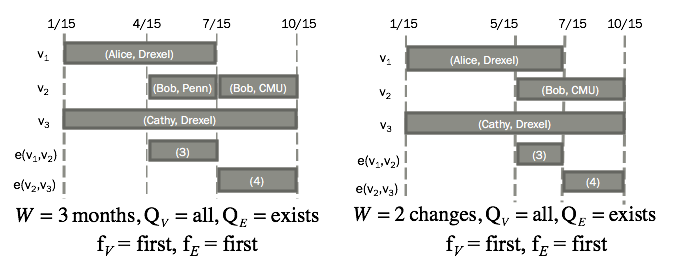
\includegraphics[width=5in]{figs/agg.png}
\caption{Temporal aggregation over \insql{T1} (Figure~\ref{fig:tg_ve}). \julia{update}}
\label{fig:tg_agg}
\end{figure*}

{\bf Temporal aggregation may uncoalesce \tve and \trg.} Consider a
\tg \insql{T} that consists of only 1 vertex $v_1$ and no edges, and
suppose that $v_1$ exists during the odd months of the year.  That is,
\tv contains $(v_1, [1/16, 2/16)), \ldots,$ $(v_1, [11/16,12/16))$,
    for which time periods do not meet and so these tuples cannot be
    coalesced.  Next consider $\tve'$ in the result of
    $\gamma_{W=2~months, Q_V=exists,Q_E=all}(T)$.  This relation will
    contain $(v_1, [1/16, 3/16)), \ldots,$ $,(v_1, [11/16,1/17))$ ---
        one tuple per input tuple, all tuples meet and so \tv' must be
        coalesced.  A similar argument holds for other relations of
        \tve, and for \trg.

{\bf Temporal aggregation requires FK enforcement for \tve.}  As
illustrated in Figure~\ref{fig:tg_agg}, $(v_1,v_2,[1/15,5/15))$ is
  removed from $\te'$ not because it did not exist at some point
  during $[1/15,5/15)$ but because $(v_2,[1/15,5/15))$ is absent from
      $\tv'$.  

We now give an analysis of whether FK enforcement is required, by
considering the relationship between vertex and edge aggregation
quantifiers $Q_V$ and $Q_E$.  Recall that we support quantifiers
\insql{all}, \insql{most}, \insql{at least} $n$, and \insql{exists},
and observe that they can be translated to a threshold on the
percentage of the time during which an entity (vertex or edge)
existed, relative to the duration of the aggregation window: $t = 1$
for \insql{all}, $t > 0.5$ for \insql{most}, $t > 0$ for
\insql{exists} and $t > n$ for \insql{at least} $n$.  Let us refer to
the vertex threshold as $t_V$, and to the edge threshold as $t_E$.  If
an entity's existence meets the threshold, it will be retained in the
result of aggregation.

\julia{rewrite} FK enforcement is only required if $t_V$ is stricter
than $t_E$.  To see why, consider 2 cases.  (1) Suppose that $t_V \leq
t_E$.  To violate FK constraint, we must produce edge $(v_1, v_2, p)
\in \te'$ and not produce vertex $(v_1, p) \in \tv'$.  This edge
$(v_1, v_2)$ must have been valid during at least $t_E$ portion of p
in \te.  If our input is valid, then there must exist both $v_1$ and
$v_2$ in \tv during at least $t_E$ portion of p to pass the FK
constraint.  Since $t_E$ is at least as large as $t_V$, we will
produce both $(v_1, p)$ and $(v_2, p)$.  (2) $t_V > t_E$.  The proof
here is similar to above.  If we produce edge $(v_1, v_2, p) \in
\te'$, then there must be both $v_1$ and $v_2$ in \tv that exist
during at least $t_V$ portion of p.  However, since $t_V$ is larger
than $t_E$, we may not produce a vertex in \tv' that meets $t_E$ but
does not meet the greater $t_V$.  In that case the edge is violating
the FK constraint.

\eat{ Our aggregation quantifiers are inspired by generalized
  quantifiers of~\cite{Hsu1995} with n-place delimiters.  $Q(R)$ as a
  Boolean-valued function of a relation''~\cite{Hsu1995}.  A
  quantifier contains an n-place determiner, e.g., ``at least one
  vertex in each window for each group'' is a 2-place determiner
  quantifier.  \tg algebra supports determiners from the set
  $\{at\ least\ one, all, most, at\ least\ n\}$, where $n$ is an
  integer representing a ratio.  $all$ is a usual universal quantifier
  that in standard SQL can be achieved with the use of two \insql{NOT
    EXISTS}.}

\eat{Aggregation in relational algebra produces results for each grouping
irrespective of how many results there are, unless a \insql{HAVING}
restriction is applied.  The quantification over the aggregation
results in evolving graphs is useful for producing different kinds of
representative graphs.  For example, to produce a representative graph
with only strong connections over a volatile evolving graph, we want
to restrict results to those edges that span the entire window or a
large subset of that window.  For this purpose we introduce
quantifiers.}

\eat{
The second observation is that it is necessary to enforce referential
integrity.  Consider a pair of relations $R_i, R_j \in T_{VE}$, such
that there is a foreign key on $R_j$ referencing $R_i$, and consider
the counterparts of these relations $R'_i = \sigma_{c_i} R_i$ and $R'_j
= \sigma_{c_j} R_j$.  If the selection condition on $R_i$ is trivial
(i.e., $R_i = \sigma_{c_i} R_i$), then referential integrity will hold
on $R_i, R_j$.  However, if $c_i$ removes some tuples from $R_i$, then
it becomes necessary to idenfity tuples in $R'_j$ for which there is
no counterpart in $R'_i$ and delete them.}

\eat{
Recall that a \tg is a pair of coalesced temporal SQL relations, with
an integrity constraint that ensures that an edge exists at a time
when both vertices it connects also exist.  We start by investigating
the behavior of our model under a standard definition of temporal
relational algebra operators applied to $V$, $E$ or both in
Section~\ref{sec:algebra:rel}.  We then present the novel operations
of \tg algebra (Section~\ref{sec:algebra:graph}).  The main challenge
in both sub-section is understanding whether and when to coalesce $V$
and $E$, and how to efficiently enforce the integrity of the data
structure.}

%\subsection{Relational algebra operators over $V$ and $E$}

\eat{$V$ and $E$ are valid-time temporal relations, and we adopt (and
adapt) the semantics of period-based temporal
algebra~\cite{DBLP:conf/vldb/BohlenSS96} to our setting. }

\eat{1) Apply operation to V
2) Apply operation to E
3) Coalesce V if necessary
4) Coalesce E is necessary
5) Enforce integrity constraint}

\eat{Temporal selection $\sigma_c V = \{ \langle v, p, a_1, \ldots, a_n
\rangle | c(\langle v, p, a_1, \ldots, a_n \rangle) \}$ returns a
subset of the tuples in $V$. Note that the selection condition $c$ is
an arbitrary Boolean condition that may also include predicates on
$p$.  }

\eat{When evaluated over coalesced input relations, temporal selection,
temporal Cartesian product and temporal negation preserve coalescing.}

\eat{
\begin{definition}[Selection]
Temporal and structural selection on $TG$ is a selection on the
attributes of $V$ and $E$, including entity periods.  $\sigma_{a
  \theta c}(TG)$, where $a$ are attributes of $V$ and/or $E$,
including periods, $\theta$ is a binary operation in the set $\{<,
\leq, =, \neq, \geq, >\}$, and $c$ is a value constant.
\label{def:selection}
\end{definition}}

\eat{Temporal and structural selection are supported by the same selection
operator and can be used together.  For example, one could select a
sub-graph in an evolving co-citation network of only authors whose
names start with letter A, over the past decade.  Because of the
constraint on $E$, even if the structural selection is only on
attributes of $V$, only edges connecting selected vertices are
retained.  Neither deduplication nor coalescing is required as a
post-operation.  Note that temporal selection and slice are different
because temporal selection does not modify entity periods, only
selects some of them.}

\eat{In SQL, selection can be expressed as a regular selection on V,
followed by a selection on E with integrity constraint enforced.}

\eat{\begin{definition}[Projection]
Projection on $TG$ is projection on attributes of $V$ and $E$ with
coalescing, i.e. \\$\Pi vid, p, a_1, \ldots, a_n(V); \Pi vid_1, vid_2,
p, b_1, \ldots, b_m(E)$. 
\label{def:projection}
\end{definition}}

\eat{\begin{definition}[Slice]
The unary operation \op{slice}, denoted $\sigma_{[start, end)}
  \insql{T}$ is a selection operation that includes...}

\eat{Slice on $TG$ is a selection on periods of $V$ and $E$ such that
$slice_{[a,b)}(TG) = \{t': t \in TG$, $t(p).overlaps(period(a,b)), t'
  = fit(t, period(a,b))\}$ and $fit(t, period(a,b))$ shortens the
  entity period $p$ to be within $[a,b)$.
\label{def:slice}
\end{definition}}

\eat{In SQL, slice can be expressed as follows for $V$
(similarly for $E$):}

\eat{\begin{small}
\begin{verbatim}
SELECT vid, a1, ..., an, greatest(estart, DATE ':date1'), 
       least(eend, DATE ':date2')
FROM V
WHERE eperiod OVERLAPS PERIOD (DATE ':date1', DATE ':date2')
\end{verbatim}
\end{small}}

%\subsection{Temporal aggregation}

\eat{Now that we have the window semantics and quantification defined, we
can define the aggregation operation over an evolving graph $TG$.}

\eat{It is often useful to analyze aggregate behavior of an evolving graph
over some coarser time period.  For example, a union of all
vertices/edges over 1 month is representative of that graph during
that month.  Analysis of aggregate behavior can lead to deeper insight
than of a snapshot.  For example, a co-authorship network DBLP is very
sparse --- one can only publish so many papers in any given month ---
on a daily or even monthly level of granularity, but can show
community formation and affiliation when aggregated over multiples of
years.  From this perspective, an evolving graph is a sequence of
representative graphs over consecutive arbitrary-length periods.}

\eat{
\begin{definition}[\tg Aggregation]
An {\em aggregation} operation over $TG$ is a function \\ $G_1, G_2,
\ldots, G_n, W, Q g f_1(A_1), f_2(A_2), \ldots, f_m(A_m)(TG)$, where
each $G_i$ is a grouping attribute from $TG$ with the exception of
$p$; $W$ is the window specification; $Q$ is a generalized quantifier
specification for vertices and edges on the coverage of the window;
each $F_i$ is an aggregation function; and each $A_i$ is an attribute
name from $TG$.
\label{def:agg}
\end{definition}}

\eat{This definition is similar to the regular relational algebra
aggregation definition, with the addition of the window specification
and the restriction of grouping attributes to exclude the time
periods.  However, both $V$ and $E$ relations are aggregated by the
same operation and the constraint on $E$ to contain only those
vertices that exist in $V$ is maintained.  The aggregation defined
this way allows to aggregate graphs structurally, temporally, or in
combination.  To aggregate only temporally, the grouping attribute
must be $vid$ for $V$ and $(vid1, vid2)$ for $E$.  To aggregate only
structurally, the window specification must be by 1 change.  Observe
that aggregation by 1 change with grouping by id is a no-op, and in
fact the sequence of representative graphs on the source data is equal
to the deduplicated sequence of snapshots.}

\eat{The quantifier is applied to the coverage of the window period
  within each grouping.  For example, to construct the persistent
  edges graph from the example above, we use the $all$ quantifier over
  the $E$ relation.  Only the edges that span the duration of the
  window period are produced.  Since the universal quantification is
  very restrictive, $most$ and $at\ least\ n$ quantifiers are more
  appropriate in some aggregations, especially over long windows.  To
  obtain a stable 1-month graph over an evolving network connections
  graph, we may ask for connections that exist in at least 90\% of the
  period.}

\eat{Remember that the schema for $V$ has a $(vid, p)$ primary key.  Any
aggregation operation must produce both a valid $vid$ and valid time
interval for each tuple.  We produce a $vid$ by using the hash of the
grouping variables to maintain temporal consistency.  The time
interval is produced by the window extent from the window
specification. Similarly for $E$.}

\eat{The aggregation functions over the selected graph attributes are used
to compute the new value representative of the whole window.  We
support the standard set $\{count, min,$ $max, sum, average\}$, as
well as $\{any, first, last, list\}$.  $first$ and $last$ refer to
first/last non-null value in the window and are possible because the
aggregating tuples have the time dimension, and the ties are decided
arbitrarily.  $count$ is the count of the number of distinct values
over the aggregation window.  Additional aggregation functions can be
defined by the user.}

\eat{\begin{figure*}
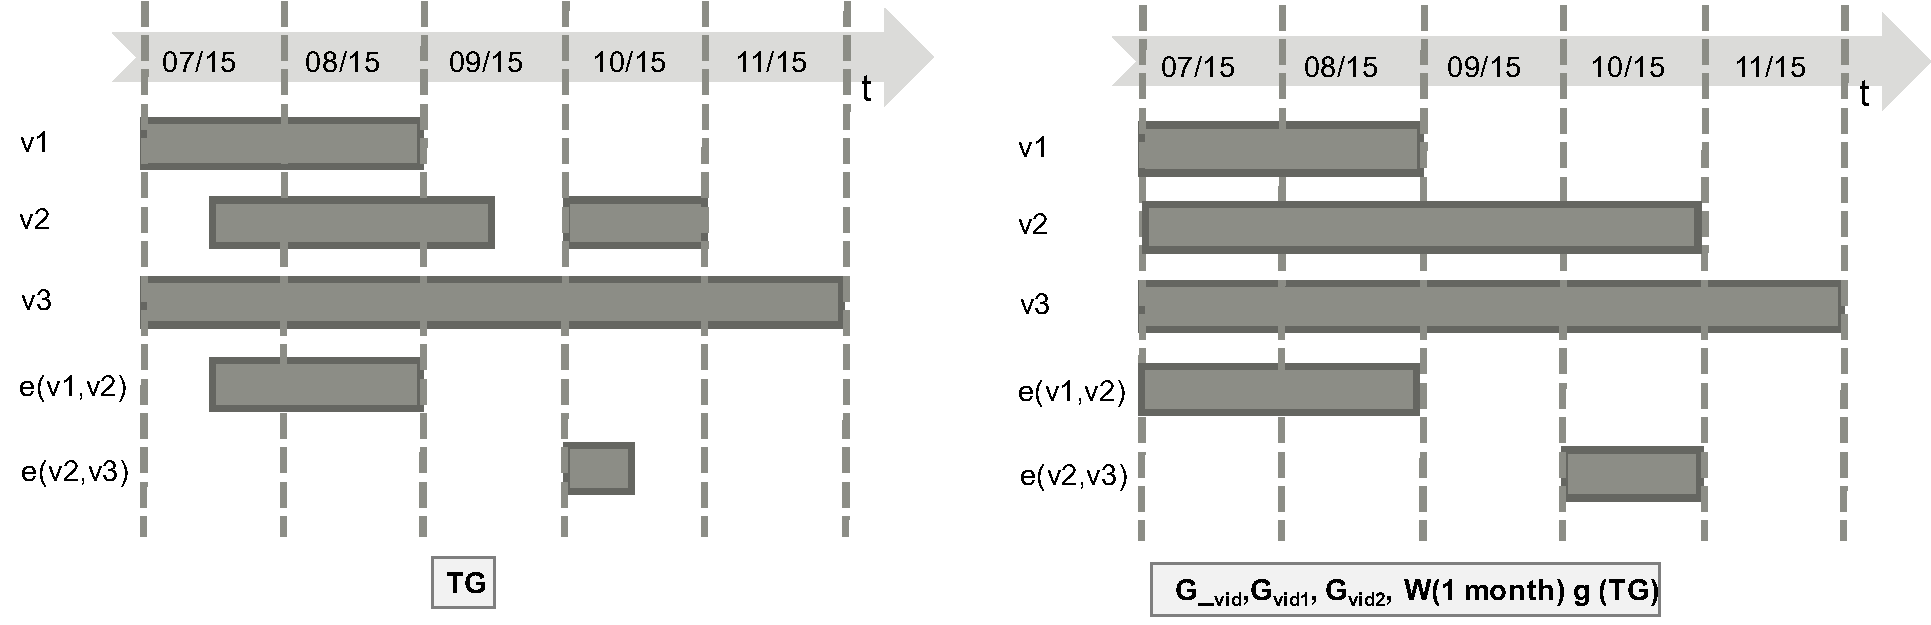
\includegraphics[width=6.5in]{figs/agg1.pdf}
\caption{1-month window aggregation with grouping by id, with
  existential vertex/edge quantifier.  Structure only.}
\label{fig:agg1}
\end{figure*}
}

\eat{An example in Figure~\ref{fig:agg1} shows a small \tg and a result of
aggregation by 1 month on that graph with $at\ least\ one$ quantifier,
with group by id.}

\subsection{Temporal graph intersection}
\label{sec:algebra:join}

The binary temporal graph intersection operation $\trga \cap \trgb$
computes a temporal join~\cite{Gao2005} of \trga and \trgb with the
predicate $\trga.p \cap \trgb.p \neq \emptyset$, producing a tuple for
each pair of representative graphs for which time periods intersect:
$\trga \cap \trgb = \{(g_1 \cap g_2, p_1 \cap p_2)~|~((g_1, p_1) \in
\trga \wedge (g_2, p_2) \in \trgb \wedge p_1 \cap p_2 \neq \emptyset
\}$.  The result of $g_1 \cap g_2$ is computed by intersecting the
sets of vertices and of edges of the graphs~\cite{GraphTheory}.  For
each vertex and edge in the result, we compute a {\em union} of their
bags of properties. \julia{Figure with example.}

\eat{The computation over \trg is essentially a temporal inner
  theta-join of $\trg_1$ and $\trg_2$ with a $p_1 \cap p_2$ predicate,
  followed by projection of $p_1, p_2$ into $p_1 \cap p_2$.  We use
the standard graph intersection definition based on set theory, which
intersects the vertex and edge sets from the two
operands~\cite{GraphTheory}.}

Algorithm~\ref{alg:inter} presents the evaluation of $\tvea \cap
\tveb$.  We compute temporal joins over the corresponding \tv and \te
relations (lines 1, 2).  We then compute \tav' and \tae' by performing
temporal outer joins of the corresponding relations (lines 3, 4).
Finally, we enforce foreign key constraints on \te', \tav' and \tae'
(lines 5, 6).

\begin{algorithm}
\caption{Temporal graph intersection in \tve.}
\begin{algorithmic}[1]
%\REQUIRE $\tvea (\tv_1;\te_1;\tav_1;\tae_1), \tveb (\tv_2;\te_2;\tav_2;\tae_2)$.\\
\REQUIRE $\tvea, \tveb$.\\
\STATE $\tv' = \cl (\tv_1 \Join^T_v \tv_2)$\\
\STATE $\te' = \cl (\te_1 \Join^T_{v_1,v_2} \te_2)$\\
\STATE $\tav' = \pi_{v,p,\tav_1.a \cup \tav_2.a}\tav_1 \fullouterjoin^T_v \tav_2$\\
\STATE $\tae' = \pi_{v_1,v_2,p,\tae_1.a \cup \tae_2.a}\tae_1 \fullouterjoin^T_{v_1,v_2} \tae_2$\\
%\STATE $\tae' = \pi_{a_1 \cap a_2}(\tae_1 \Join^T \tae_2)$\\
\STATE  enforce foreign keys on $\tav'$ w.r.t. $\tv'$\\
\STATE  enforce foreign keys on $\tae'$ w.r.t. $\te'$\\
\RETURN new $\tve (\tv';\te';\tav';\tae')$\\
\end{algorithmic}
\label{alg:inter}
\end{algorithm}

{\bf Intersection may uncoalesce \tve and \trg.}  While temporal join over
coalesced temporal relations does not uncoalesce, as shown
in~\cite{DBLP:conf/vldb/BohlenSS96}, it is followed by a projection,
which does uncoalesce.  For example, consider a simple \tg $T_2$
that consists of only 1 vertex $v_1$ with attribute $(name:Alice)$ and
no edges and exists for the period $[1/15, 5/15)$.  The
  intersection of $T_2$ with \insql{T} in Figure~\ref{fig:tg_rg}
  produces the same graph with vertex $v_1$ for each period of
  intersection $[1/15, 2/15), [2/15, 5/15)$, which must be coalesced.

{\bf Intersection requires FK enforcement for \tav and \tae but not
  for \te.}  \julia{revise} The proof for this is similar to the one
for \insql{slice}.  Consider an edge $\te(v_1, v_2, p^e)$ and one of
the corresponding vertices $\tv(v_1, p^v)$ obtained through temporal
joins above.  To violate the FK constraint, there has to exist at
least one time instant $t \in p^e \wedge t \not\in p^v$.  But that is
not possible, since by definition of temporal join $p^e$ exists both
in $\te_1$ and $\te_2$ and $\tve_1$ and $\tve_2$ are valid \tgs.

\subsection{Temporal graph union}
\label{sec:algebra:outerjoin}

The binary temporal graph union operation $\trga \cup \trgb$ computes
a temporal full outer join~\cite{Gao2005} of \trga and \trgb on the
predicate $\trga.p \cap \trgb.p $. For tuples $(g_1, p_1) \in \trga$
and $(g_2, p_2) \in \trgb$ for which $p_1 \cap p_2 \neq \emptyset$, we
compute $(g_1 \cup g_2, p_1 \cap p_2)$.  The result of $g_1 \cup g_2$
is computed by taking a {\em union} of the sets of vertices and of
edges of the graphs~\cite{GraphTheory}.  For each vertex and edge in
the result, we compute a {\em union} of their bags of properties.
Tuples from \trga (resp. \trgb)for which there does not exist a tuple
in \trgb (resp. \trga) for part or all of the validity period are
included in the result of the full outer join.  \julia{Figure with
  example.}

\eat{
 $\trg_1 \cup \trg_2 = \{ (g, p) | (g_1, p_1) \in \trg_1 \wedge (g_2,
p_2) \in \trg_2 \wedge ((g = g_1 \cup g_2 \wedge p = p_1 \cap p_2
\wedge p_1 \cap p_2 \neq \emptyset) \vee (g = g_1 \wedge p = p_1 - p_2
\wedge \nexists p \in \trg_2 = p_1 - p_2) \vee (g = g_2 \wedge p = p_2
- p_1 \wedge \nexists p \in \trg_1 = p_2 - p_1))\}$.  Similar to
temporal intersection, temporal union is essentially an outer
theta-join of $\trg_1$ and $\trg_2$ with a $p_1 \cap p_2$ predicate.
We use the standard graph union definition based on set theory, which
computes unions of the vertex and edge sets from the two
operands~\cite{GraphTheory}.}

Algorithm~\ref{alg:union} presents the evaluation of $\tvea \cup
\tveb$.  We compute temporal joins over the corresponding \tv and \te.

\begin{algorithm}
\caption{Temporal graph union in \tve.}
\begin{algorithmic}[1]
\REQUIRE $\tvea, \tveb$.\\
\STATE $\tv' = \cl (\tv_1 \fullouterjoin^T_v \tv_2)$\\
\STATE $\te' = \cl (\te_1 \fullouterjoin^T_{v1,v2} \te_2)$\\
\STATE $\tav' = \pi_{v,p,\tav_1.a \cup \tav_2.a}\tav_1 \fullouterjoin^T_v \tav_2$\\
\STATE $\tae' = \pi_{v_1,v_2,p,\tae_1.a \cup \tae_2.a}\tae_1 \fullouterjoin^T_{v1,v2} \tae_2$\\
\RETURN new $\tve (\tv';\te';\tav';\tae')$\\
\end{algorithmic}
\label{alg:union}
\end{algorithm}

\eat{\begin{algorithm}
\caption{Temporal graph union in \tve.}
\begin{algorithmic}[1]
\REQUIRE $\tve_1 (\tv_1, \te_1, \tav_1, \tae_1), \tve_2 (\tv_2, \te_2, \tav_2, \tae_2)$.\\
\STATE $\tv' = \tv_1 \fullouterjoin^T \tv_2$\\
\STATE $\te' = \te_1 \fullouterjoin^T \te_2$\\
\STATE $\tav' = \pi_{a_1 \cup a_2}(\tav_1 \fullouterjoin^T \tav_2)$\\
\STATE $\tae' = \pi_{a_1 \cup a_2}(\tae_1 \fullouterjoin^T \tae_2)$\\
\RETURN new $\tve (\tv', \te', \tav', \tae')$\\
\end{algorithmic}
\label{alg:union}
\end{algorithm}
}

{\bf Union may uncoalesce \tve and \trg.}  The logic here is similar
to the case with temporal intersection.  Because we produce a single
graph for each time period by computing a union of $g_1$ and $g_2$, a
form of projection, the result may be uncoalesced.  For example,
consider a simple \tg $T_2$ that consists of a single graph equal to
the first representative graph of \insql{T} in Figure~\ref{fig:tg_rg}
valid for a period of $[12/14, 5/15)$.  The same representative graph
  will be produced for period $[12/14, 1/15)$ and $[1/15, 2/15)$ and
      must be coalesced.  \julia{can this operation uncoalesce \tav
        and \tae or only \tv and \te?  Explain, modify lines 3, 4 of
        algorithm if yes.}

{\bf Union does not require FK enforcement for \tve.}
\julia{rephrase, ``remove'' is not the right explanation, the result
  is a new graph.} A full outer join does not remove any vertices or
edges from either $\trg_1$ or $\trg_2$, so the validity of all
resulting edges remains intact.

\eat{\begin{definition}[Union] Union of $TG1\ \cup\ TG2$ = $\{v, e: v
    \in TG1.V$ or $v \in TG2.V$ or $v(vid$, $f_1(a_{11}$, $a_{21})$,
    \ldots, $f_n(a_{1n}, a_{2n})$, $period(least(p_1, p_2),
    greatest(p_1, p_2)))$, $e \in TG1.E$ or $e \in TG2.E$ or $e(vid1,
    vid2, g_1(b_{11}, b_{21}), \ldots, g_m(b_{1m}, b_{2m})$,
    $period(least(p_1, p_2), greatest(p_1, p_2))) \}$, where each $f$,
    respectively $G$, is an aggregation function over one vertex,
    respectively edge, attribute where the values intersect over some
    period $p$.
\label{def:union}
\end{definition}}

\eat{\begin{figure*}
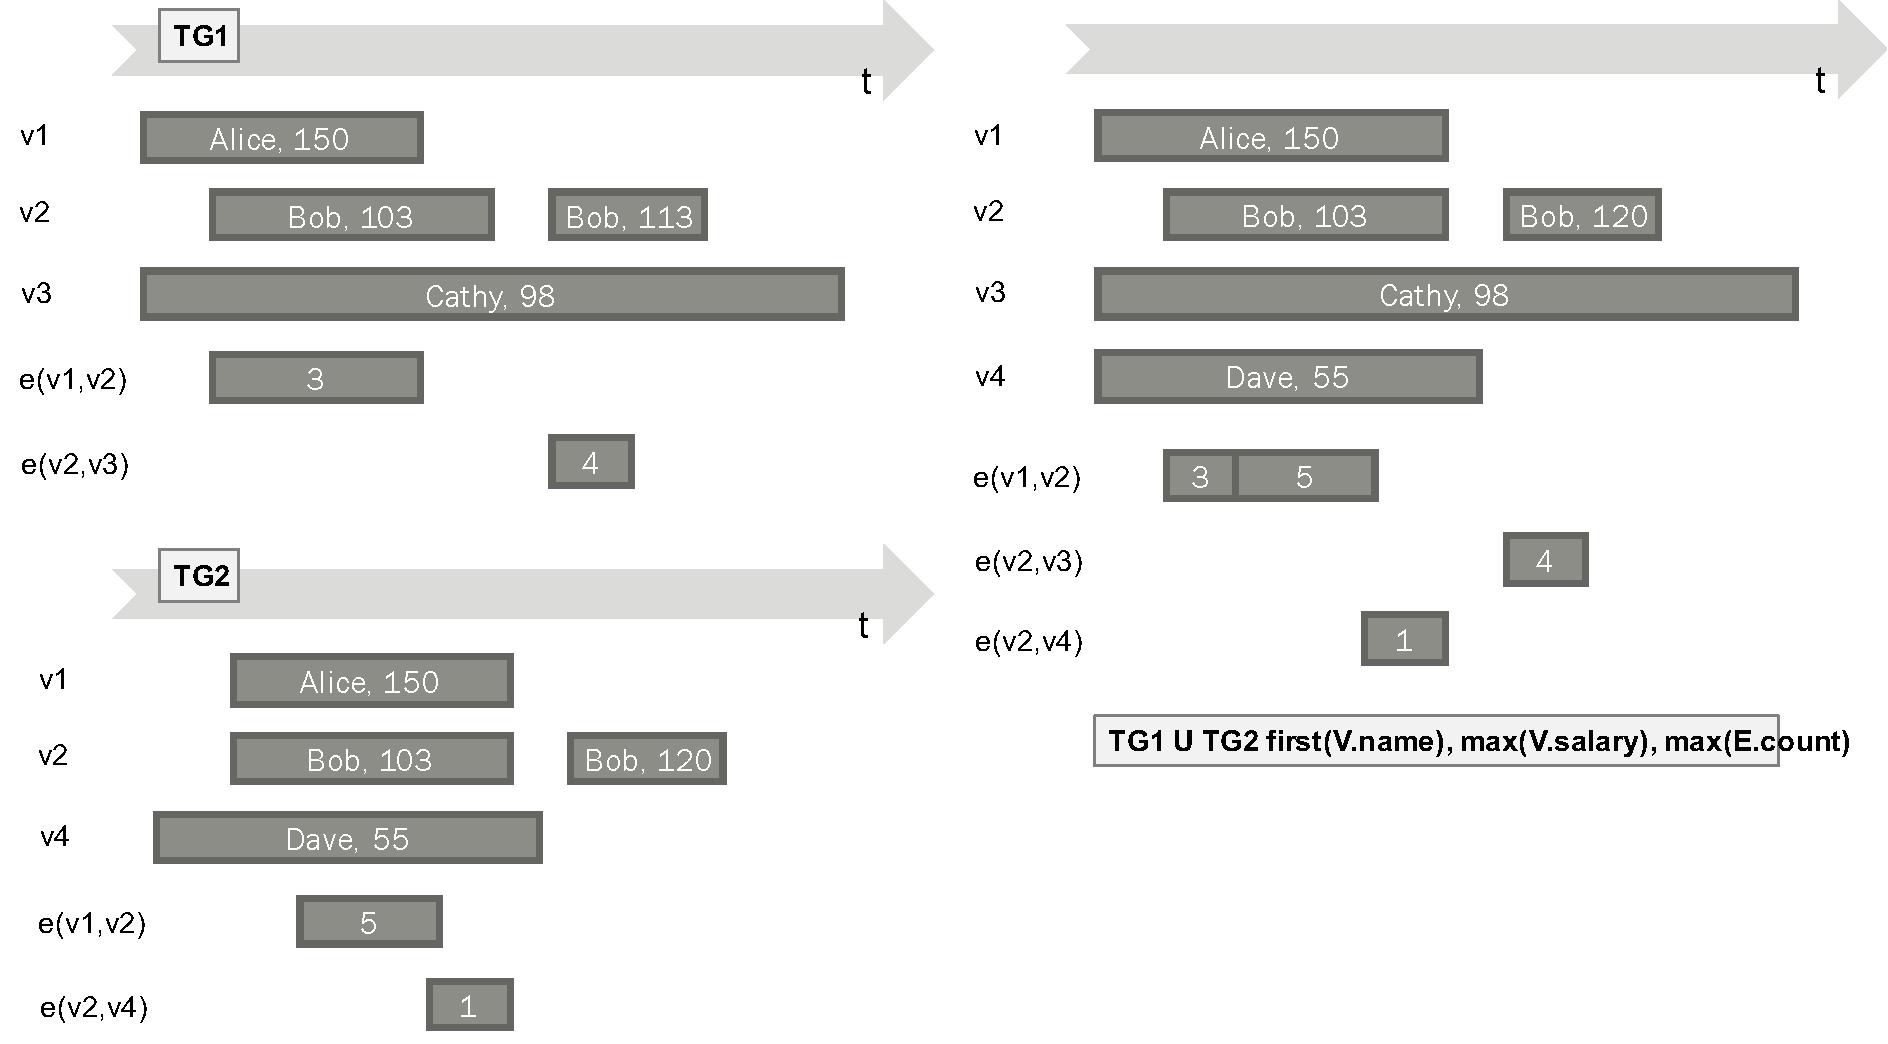
\includegraphics[width=6.5in]{figs/union.pdf}
\caption{Union of TG1 and TG2.}
\label{fig:union}
\end{figure*}}

\eat{In other words, union of two \tgs is simply all vertices and edges
from both \tgs, with vertex/edge attributes decided by specified
aggregation functions for each period where both values are present,
with coalescing.  Figure~\ref{fig:union} illustrates this concept.}

\eat{Similarly, intersection of two \tgs is an intersection of
vertices/edges of two graphs, with values for each overlapping
attribute computed by a specified aggregate function.}

\eat{So far we have defined the operations in our temporal graph
  algebra.  Next we define another class of non-algebraic operations
  on evolving graphs that are nevertheless very useful: analytics.}

\eat{\vera{What I think we are leaving out: difference, structural
  aggregation (new entity creation), graph joins and products (maybe?
  graph joins are weird), more general select (with time in predicate
  and/or path predicates), reverse/transpose.}}
